\documentclass{standalone}
\usepackage{tikz}
\usetikzlibrary{patterns, positioning}

\begin{document}
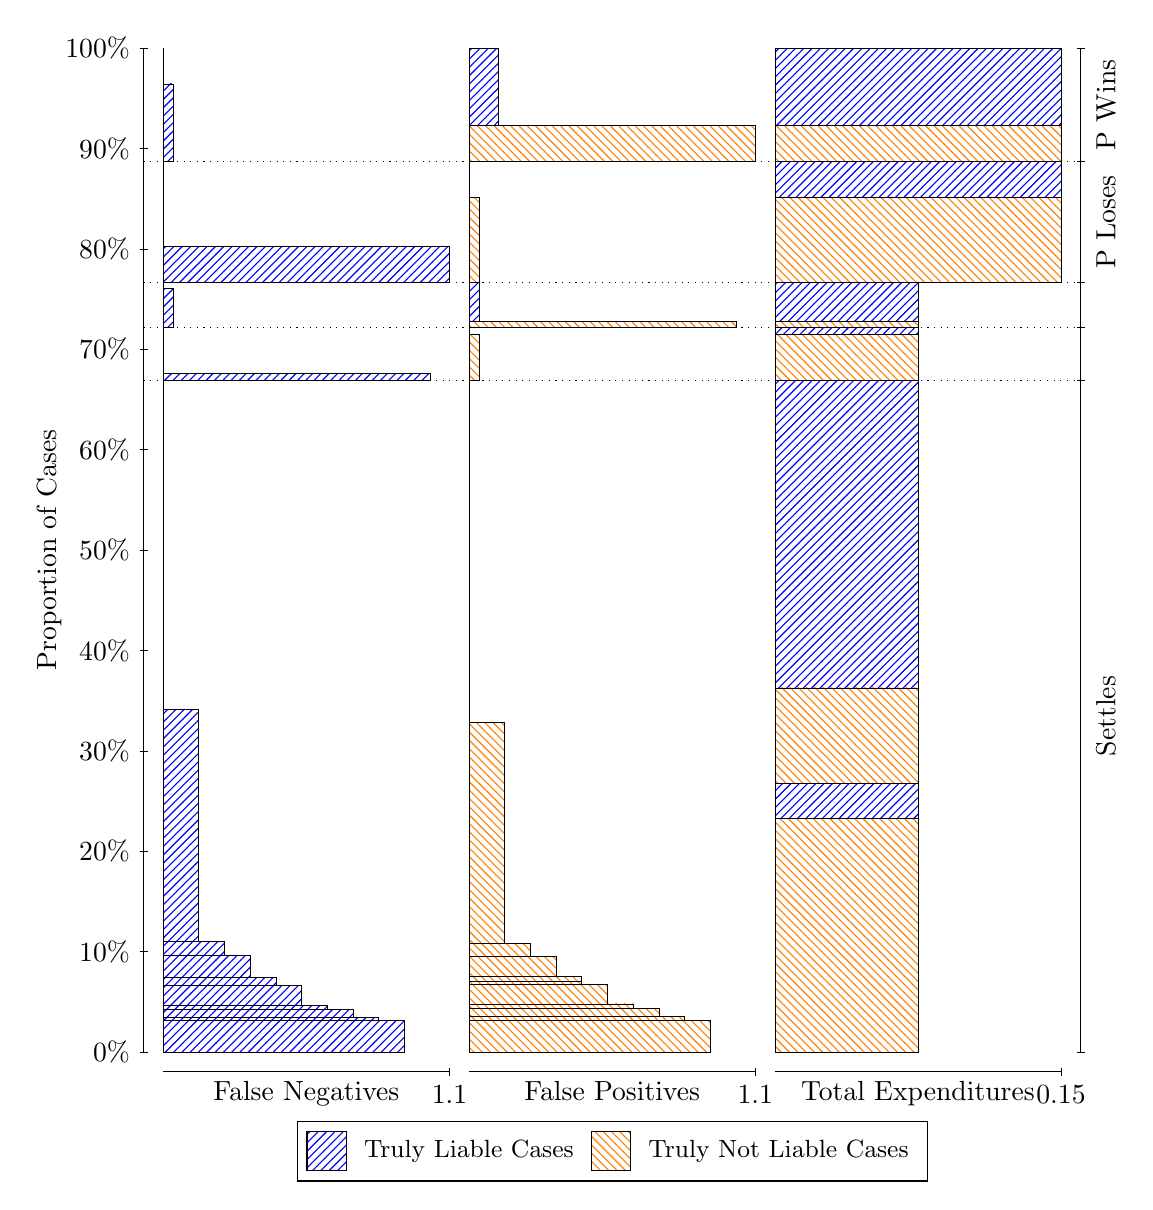
\begin{tikzpicture}
\draw[black, very thin] (1.5,1.75) -- (1.5,14.5);
\node[rotate=90, anchor=center] at (0.3, 8.125) {Proportion of Cases};
\draw[black, very thin] (1.45,1.75) -- (1.55,1.75);
\node[anchor=east] at (1.45, 1.75) {0\%};
\draw[black, very thin] (1.45,3.025) -- (1.55,3.025);
\node[anchor=east] at (1.45, 3.025) {10\%};
\draw[black, very thin] (1.45,4.3) -- (1.55,4.3);
\node[anchor=east] at (1.45, 4.3) {20\%};
\draw[black, very thin] (1.45,5.575) -- (1.55,5.575);
\node[anchor=east] at (1.45, 5.575) {30\%};
\draw[black, very thin] (1.45,6.85) -- (1.55,6.85);
\node[anchor=east] at (1.45, 6.85) {40\%};
\draw[black, very thin] (1.45,8.125) -- (1.55,8.125);
\node[anchor=east] at (1.45, 8.125) {50\%};
\draw[black, very thin] (1.45,9.4) -- (1.55,9.4);
\node[anchor=east] at (1.45, 9.4) {60\%};
\draw[black, very thin] (1.45,10.675) -- (1.55,10.675);
\node[anchor=east] at (1.45, 10.675) {70\%};
\draw[black, very thin] (1.45,11.95) -- (1.55,11.95);
\node[anchor=east] at (1.45, 11.95) {80\%};
\draw[black, very thin] (1.45,13.225) -- (1.55,13.225);
\node[anchor=east] at (1.45, 13.225) {90\%};
\draw[black, very thin] (1.45,14.5) -- (1.55,14.5);
\node[anchor=east] at (1.45, 14.5) {100\%};

\draw[black, very thin] (13.4,1.75) -- (13.4,14.5);
\draw[black, very thin] (13.35,1.75) -- (13.45,1.75);
\node[anchor=west] at (13.35, 1.75) {};
\draw[black, very thin] (13.35,10.283) -- (13.45,10.283);
\node[anchor=west] at (13.35, 10.283) {};
\draw[black, very thin] (13.35,10.95) -- (13.45,10.95);
\node[anchor=west] at (13.35, 10.95) {};
\draw[black, very thin] (13.35,11.523) -- (13.45,11.523);
\node[anchor=west] at (13.35, 11.523) {};
\draw[black, very thin] (13.35,13.057) -- (13.45,13.057);
\node[anchor=west] at (13.35, 13.057) {};
\draw[black, very thin] (13.35,14.5) -- (13.45,14.5);
\node[anchor=west] at (13.35, 14.5) {};

\draw[black, very thin, pattern color=blue, pattern=north east lines] (1.75,1.75) rectangle (4.8118,2.148);
\draw[black, very thin, pattern color=blue, pattern=north east lines] (1.75,2.148) rectangle (4.4852,2.1917);
\draw[black, very thin, pattern color=blue, pattern=north east lines] (1.75,2.1917) rectangle (4.1586,2.2909);
\draw[black, very thin, pattern color=blue, pattern=north east lines] (1.75,2.2909) rectangle (3.832,2.3411);
\draw[black, very thin, pattern color=blue, pattern=north east lines] (1.75,2.3411) rectangle (3.5054,2.5956);
\draw[black, very thin, pattern color=blue, pattern=north east lines] (1.75,2.5956) rectangle (3.1788,2.6968);
\draw[black, very thin, pattern color=blue, pattern=north east lines] (1.75,2.6968) rectangle (2.8522,2.9762);
\draw[black, very thin, pattern color=blue, pattern=north east lines] (1.75,2.9762) rectangle (2.5257,3.1546);
\draw[black, very thin, pattern color=blue, pattern=north east lines] (1.75,3.1546) rectangle (2.1991,6.102);
\draw[black, very thin, pattern color=orange, pattern=north west lines] (1.75,6.102) rectangle (1.75,10.283);
\draw[black, very thin, pattern color=blue, pattern=north east lines] (1.75,10.283) rectangle (5.1384,10.367);
\draw[black, very thin, pattern color=orange, pattern=north west lines] (1.75,10.367) rectangle (1.75,10.95);
\draw[black, very thin, pattern color=blue, pattern=north east lines] (1.75,10.95) rectangle (1.8725,11.446);
\draw[black, very thin, pattern color=orange, pattern=north west lines] (1.75,11.446) rectangle (1.75,11.523);
\draw[black, very thin, pattern color=blue, pattern=north east lines] (1.75,11.523) rectangle (5.3833,11.98);
\draw[black, very thin, pattern color=orange, pattern=north west lines] (1.75,11.98) rectangle (1.75,13.057);
\draw[black, very thin, pattern color=blue, pattern=north east lines] (1.75,13.057) rectangle (1.8725,14.044);
\draw[black, very thin, pattern color=orange, pattern=north west lines] (1.75,14.044) rectangle (1.75,14.5);
\draw[black, very thin, pattern color=orange, pattern=north west lines] (5.6333,1.75) rectangle (8.6951,2.1538);
\draw[black, very thin, pattern color=orange, pattern=north west lines] (5.6333,2.1538) rectangle (8.3685,2.2);
\draw[black, very thin, pattern color=orange, pattern=north west lines] (5.6333,2.2) rectangle (8.0419,2.3066);
\draw[black, very thin, pattern color=orange, pattern=north west lines] (5.6333,2.3066) rectangle (7.7154,2.3604);
\draw[black, very thin, pattern color=orange, pattern=north west lines] (5.6333,2.3604) rectangle (7.3888,2.6128);
\draw[black, very thin, pattern color=orange, pattern=north west lines] (5.6333,2.6128) rectangle (7.0622,2.6429);
\draw[black, very thin, pattern color=orange, pattern=north west lines] (5.6333,2.6429) rectangle (7.0622,2.7052);
\draw[black, very thin, pattern color=orange, pattern=north west lines] (5.6333,2.7052) rectangle (6.7356,2.9609);
\draw[black, very thin, pattern color=orange, pattern=north west lines] (5.6333,2.9609) rectangle (6.409,3.1264);
\draw[black, very thin, pattern color=orange, pattern=north west lines] (5.6333,3.1264) rectangle (6.0824,5.9315);
\draw[black, very thin, pattern color=blue, pattern=north east lines] (5.6333,5.9315) rectangle (5.6333,10.283);
\draw[black, very thin, pattern color=orange, pattern=north west lines] (5.6333,10.283) rectangle (5.7558,10.867);
\draw[black, very thin, pattern color=blue, pattern=north east lines] (5.6333,10.867) rectangle (5.6333,10.95);
\draw[black, very thin, pattern color=orange, pattern=north west lines] (5.6333,10.95) rectangle (9.0217,11.027);
\draw[black, very thin, pattern color=blue, pattern=north east lines] (5.6333,11.027) rectangle (5.7558,11.523);
\draw[black, very thin, pattern color=orange, pattern=north west lines] (5.6333,11.523) rectangle (5.7558,12.6);
\draw[black, very thin, pattern color=blue, pattern=north east lines] (5.6333,12.6) rectangle (5.6333,13.057);
\draw[black, very thin, pattern color=orange, pattern=north west lines] (5.6333,13.057) rectangle (9.2667,13.514);
\draw[black, very thin, pattern color=blue, pattern=north east lines] (5.6333,13.514) rectangle (6.0007,14.5);
\draw[black, very thin, pattern color=orange, pattern=north west lines] (9.5167,1.75) rectangle (11.333,4.7206);
\draw[black, very thin, pattern color=blue, pattern=north east lines] (9.5167,4.7206) rectangle (11.333,5.1623);
\draw[black, very thin, pattern color=orange, pattern=north west lines] (9.5167,5.1623) rectangle (11.333,6.3731);
\draw[black, very thin, pattern color=blue, pattern=north east lines] (9.5167,6.3731) rectangle (11.333,10.283);
\draw[black, very thin, pattern color=orange, pattern=north west lines] (9.5167,10.283) rectangle (11.333,10.867);
\draw[black, very thin, pattern color=blue, pattern=north east lines] (9.5167,10.867) rectangle (11.333,10.95);
\draw[black, very thin, pattern color=orange, pattern=north west lines] (9.5167,10.95) rectangle (11.333,11.027);
\draw[black, very thin, pattern color=blue, pattern=north east lines] (9.5167,11.027) rectangle (11.333,11.523);
\draw[black, very thin, pattern color=orange, pattern=north west lines] (9.5167,11.523) rectangle (13.15,12.6);
\draw[black, very thin, pattern color=blue, pattern=north east lines] (9.5167,12.6) rectangle (13.15,13.057);
\draw[black, very thin, pattern color=orange, pattern=north west lines] (9.5167,13.057) rectangle (13.15,13.514);
\draw[black, very thin, pattern color=blue, pattern=north east lines] (9.5167,13.514) rectangle (13.15,14.5);
\draw[black, dotted] (1.5,10.283) -- (13.4,10.283);
\draw[black, dotted] (1.5,10.95) -- (13.4,10.95);
\draw[black, dotted] (1.5,11.523) -- (13.4,11.523);
\draw[black, dotted] (1.5,13.057) -- (13.4,13.057);
\draw[black, very thin] (1.75,1.5) -- (5.3833,1.5);
\node[anchor=north] at (3.5667, 1.5) {False Negatives};
\draw[black, very thin] (5.3833,1.45) -- (5.3833,1.55);
\node[anchor=north] at (5.3833, 1.45) {1.1};

\draw[black, very thin] (5.6333,1.5) -- (9.2667,1.5);
\node[anchor=north] at (7.45, 1.5) {False Positives};
\draw[black, very thin] (9.2667,1.45) -- (9.2667,1.55);
\node[anchor=north] at (9.2667, 1.45) {1.1};

\draw[black, very thin] (9.5167,1.5) -- (13.15,1.5);
\node[anchor=north] at (11.333, 1.5) {Total Expenditures};
\draw[black, very thin] (13.15,1.45) -- (13.15,1.55);
\node[anchor=north] at (13.15, 1.45) {0.15};

\node[black, centered, rotate=90] at (13.72, 6.0167) {Settles};


\node[black, centered, rotate=90] at (13.72, 12.29) {P Loses};
\node[black, centered, rotate=90] at (13.72, 13.779) {P Wins};

\draw (7.449999999999999,1.5) node[draw=none] (baseCoordinate) {};
\begin{scope}[align=center]
        \matrix[scale=0.5, draw=black, below=0.5cm of baseCoordinate, nodes={draw}, column sep=0.1cm]{
            \node[rectangle, draw, minimum width=0.5cm, minimum height=0.5cm, pattern=north east lines, pattern color=blue] {}; &
            \node[draw=none, font=\small] (B) {Truly Liable Cases}; &
            \node[rectangle, draw, minimum width=0.5cm, minimum height=0.5cm, pattern=north west lines, pattern color=orange] {}; &
            \node[draw=none, font=\small] (B) {Truly Not Liable Cases}; \\
            };
\end{scope}

\end{tikzpicture}
\end{document}